\documentclass{article}%
\usepackage[T1]{fontenc}%
\usepackage[utf8]{inputenc}%
\usepackage{lmodern}%
\usepackage{textcomp}%
\usepackage{lastpage}%
\usepackage[head=40pt,margin=0.5in,bottom=0.6in]{geometry}%
\usepackage{graphicx}%
%
\title{\textbf{287 presos se fugaron entre enero y agosto de 2018}}%
\author{SANDRA GUERRERO}%
\date{25/09/2018}%
%
\begin{document}%
\normalsize%
\maketitle%
\textbf{URL: }%
http://www.el{-}nacional.com/noticias/sucesos/287{-}presos{-}fugaron{-}entre{-}enero{-}agosto{-}2018\_253111\newline%
%
\textbf{Periodico: }%
EN, %
ID: %
253111, %
Seccion: %
Sucesos\newline%
%
\textbf{Palabras Claves: }%
Sucesos\newline%
%
\textbf{Derecho: }%
1.10%
, Otros Derechos: %
1.2%
, Sub Derechos: %
1.10.1, 1.2.4%
\newline%
%
\textbf{EP: }%
NO\newline%
\newline%
%
\textbf{\textit{El estudio de Una Ventana a la Libertad señala que el mayor número de evasiones ocurrió en Miranda}}%
\newline%
\newline%
%
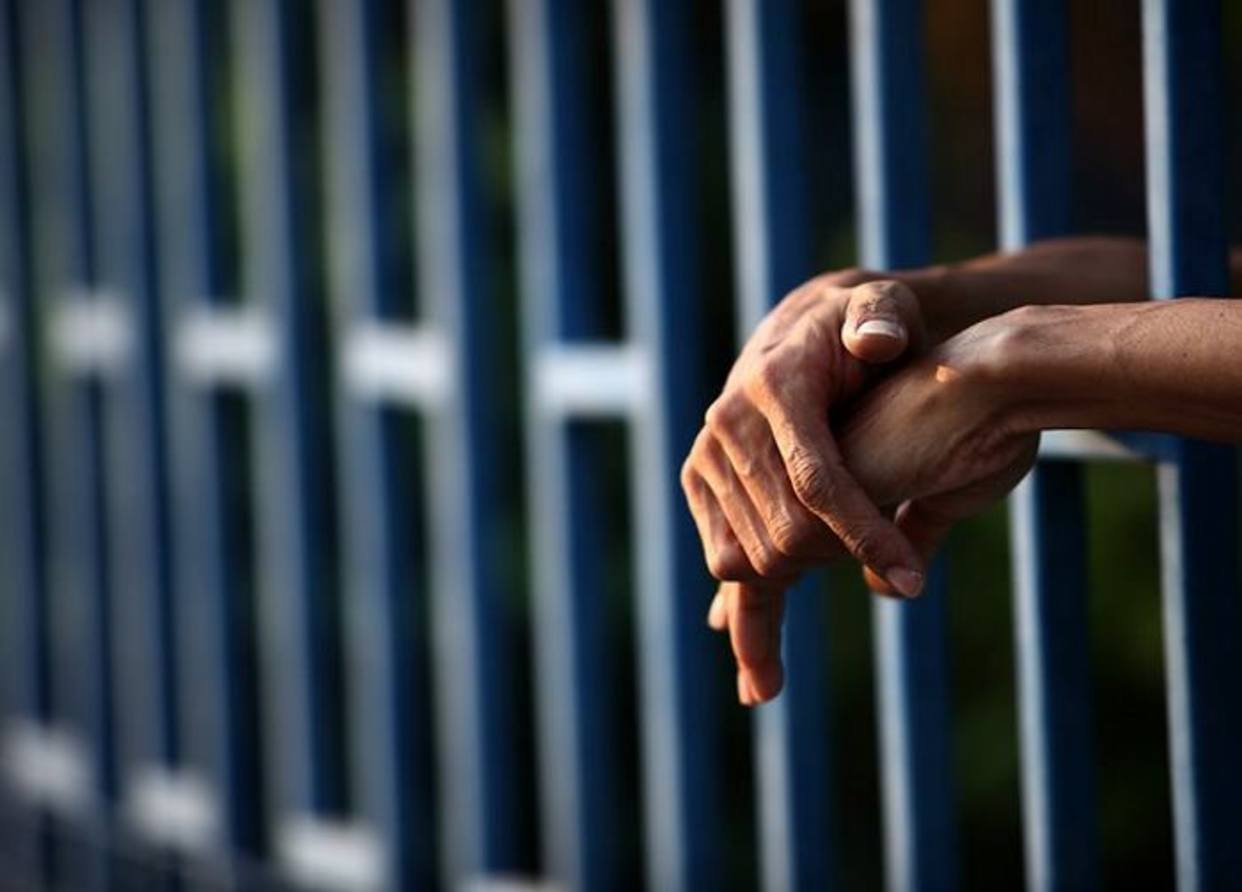
\includegraphics[width=300px]{116.jpg}%
\newline%
%
Un estudio realizado por Una Ventana a la Libertad indica que 287 privados de libertad detenidos en 93 calabozos de retenes policiales se escaparon entre enero y agosto de 2018.%
\newline%
%
La información se recabó en centros del Distrito Capital, Falcón, Bolívar, Carabobo, Mérida, Miranda, Lara, Nueva Esparta, Táchira, Monagas, Zulia y Vargas donde hubo 44 fugas.%
\newline%
%
La mayor cantidad de escapes, un total de ocho, ocurrió en Miranda. En Carabobo, Lara, Mérida, Zulia y Nueva Esparta hubo cinco en cada una de esas entidades..%
\newline%
%
La ONG señala que de los 287 presos evadidos, 269 son hombres, 94\%, y 18 mujeres para 6\%.%
\newline%
%
El informe detalla que si a esta cantidad de fugados se le restan los que luego fueron recapturados, por policías o militares, algunos con vida, otros resultaron muertos, el saldo sería de 213 privados de libertad que aún están huidos y menos de 30\% son recapturados.%
\newline%
%
El tiempo que toma concretar la recaptura es variable. Algunos casos se resuelven en horas, otros en días y algunos en más tiempo porque no es sencillo hacerles seguimiento.%
\newline%
%
A la organización le preocupa las 17 personas que fueron ultimadas en el proceso de recaptura “por parte de las autoridades policiales, en circunstancias que suelen hacer presumir uso excesivo de la fuerza”.%
\newline%
%
El estudio destaca que la mayor cantidad de evadidos que murió corresponde a Miranda, con 35\%. Luego está Zulia con 26\%; entre las dos entidades representan 61\% de todos los casos.%
\newline%
%
La recaptura de los fugados se concentra entre Nueva Esparta, 39\%, y Lara, 30\%, casi 70\% entre ambos.%
\newline%
%
“Aunque en el monitoreo realizado en este período, la cantidad de evadidos recapturados es 61 de 287, en ningún caso se conoce de algún procedimiento judicial adelantado en su contra”, indica el estudio.%
\newline%
%
A eso se agrega que en los 44 casos de fuga, al menos en 5 se pudo conocer que los funcionarios fueron detenidos por averiguación, pero no se sabe el resultado.%
\newline%
%
Investigadores de la ONG reportan en algunos estados “la presunta complicidad de funcionarios de la PNB en fugas, mediante pago de dinero”.%
\newline%
%
\end{document}